\documentclass[border={0pt 0pt 0pt 0pt}]{standalone}

\usepackage{hyperref}
\usepackage{tikz}

\usetikzlibrary{decorations.pathreplacing,
  arrows,
  calc,
  decorations.pathmorphing,
  decorations.pathreplacing,
  decorations.markings,
  fadings,
  positioning,
  shapes,
  3d
}
\usepgfmodule{oo}

\pgfdeclareradialshading{glow2}{\pgfpoint{0cm}{0cm}}{
  color(0mm)=(white);
  color(2mm)=(white);
  color(8mm)=(black);
  color(10mm)=(black)
}
\pgfdeclareradialshading{glow}{\pgfpoint{0cm}{0cm}}{
  color(0mm)=(white);
  color(5mm)=(white);
  color(9mm)=(black);
  color(10mm)=(black)
}

\begin{tikzfadingfrompicture}[name=glow fading]
  \shade [shading=glow] (0,0) circle (1);
\end{tikzfadingfrompicture}

\begin{tikzfadingfrompicture}[name=glow2 fading]
  \shade [shading=glow2] (0,0) circle (1);
\end{tikzfadingfrompicture}

\tikzstyle{snakearrow} = [decorate, decoration={pre length=0.2cm,
  post length=0.2cm, snake, amplitude=.4mm,
  segment length=2mm},thick, ->]

\ifpdf
% Ensure reproducible output
\pdfinfoomitdate=1
\pdfsuppressptexinfo=-1
\pdftrailerid{}
\hypersetup{
  pdfcreator={},
  pdfproducer={}
}
\fi

\pgfdeclarelayer{tweezer}
\pgfsetlayers{tweezer,main}
\pgfooclass{tweezer}{
  \method tweezer() {
  }
  \method drawTweezer(#1,#2,#3) {
    \begin{pgfonlayer}{tweezer}
      \shade[shading=radial,path fading=glow fading,shift={(#1,#2)},rotate=90,yscale=1,
      fill opacity=0.9,inner color=#3]
      plot[draw,samples=200,domain=-1.5:1.5] function {sqrt(0.01 + x**2 / 5)}
      -- plot[draw,samples=200,domain=1.5:-1.5] function {-sqrt(0.01 + x**2 / 5)};
    \end{pgfonlayer}
  }
  \method drawAtom(#1,#2,#3,#4) {
    \fill [#4,path fading=glow2 fading] (#1,#2) circle (#3);
  }
  \method drawNaAtom(#1,#2,#3) {
    \pgfoothis.drawAtom(#1,#2,#3,orange);
  }
  \method drawCsAtom(#1,#2,#3) {
    \pgfoothis.drawAtom(#1,#2,#3,blue);
  }
  \method drawNaTweezer(#1,#2) {
    \pgfoothis.drawTweezer(#1,#2,orange!35!black!30);
  }
  \method drawCsTweezer(#1,#2) {
    \pgfoothis.drawTweezer(#1,#2,blue!30!black!30);
  }
  \method up(#1,#2) {
    \pgfoothis.drawCsTweezer(#1,#2);
    \pgfoothis.drawNaAtom(#1,#2+0.06,0.12);
    \pgfoothis.drawCsAtom(#1,#2-0.06,0.16);
  }
  \method down(#1,#2) {
    \pgfoothis.drawCsTweezer(#1,#2);
    \pgfoothis.drawCsAtom(#1,#2+0.06,0.16);
    \pgfoothis.drawNaAtom(#1,#2-0.06,0.12);
  }
  \method naTrap(#1,#2) {
    \pgfoothis.drawNaTweezer(#1,#2);
    \pgfoothis.drawNaAtom(#1,#2,0.12);
  }
  \method csTrap(#1,#2) {
    \pgfoothis.drawCsTweezer(#1,#2);
    \pgfoothis.drawCsAtom(#1,#2,0.16);
  }
}
\pgfoonew \mytweezer=new tweezer()

\makeatletter
\def\convertto#1#2{\strip@pt\dimexpr #2*65536/\number\dimexpr 1#1}
\makeatother

\begin{document}
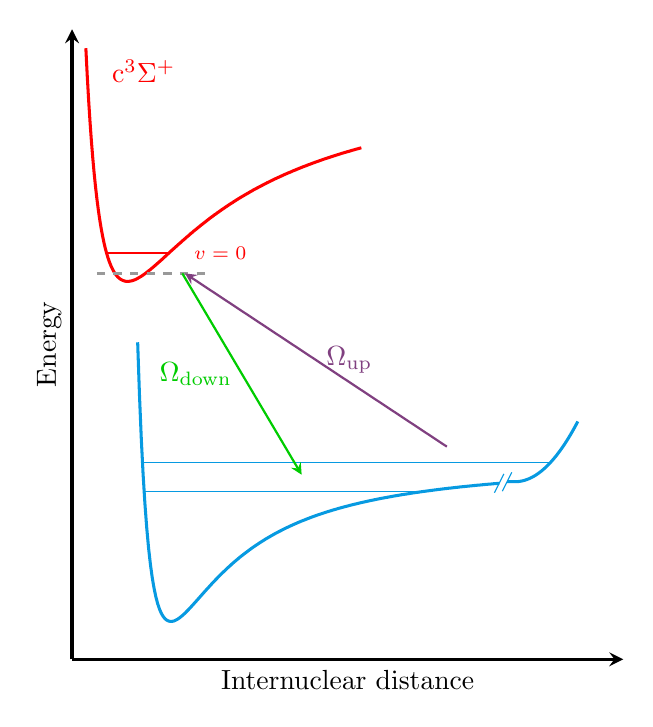
\begin{tikzpicture}
  \draw[->,>=stealth,line width=1.2] (0, 0) -- node[above,rotate=90] {Energy} (0, 8);
  \draw[->,>=stealth,line width=1.2] (0, 0) -- node[below] {Internuclear distance} (7, 0);

  \draw[line width=1.1,cyan!85!blue]
  plot[samples=200,domain=0.94:7.5,variable=\x]
  ({(\x + 0.25) * 0.7}, {(6.8*\x^(-3.4)-6.5*\x^(-1.7)) * 1.3 + 2.5}) coordinate (GroundEnd);
  \draw[cyan!85!blue] ($(GroundEnd) + (0.06, 0.12)$) -- ($(GroundEnd) - (0.06, 0.12)$);
  \draw[cyan!85!blue] ($(GroundEnd) + (0.06, 0.12) + (0.1, 0.02)$)
  -- coordinate (TrapStart) ($(GroundEnd) - (0.06, 0.12) + (0.1, 0.02)$);
  \draw[line width=1.1,cyan!85!blue]
  (TrapStart) --
  plot[samples=200,domain=0:0.8,variable=\x]
  ([shift={(TrapStart)}] {0.1 + \x}, {\x^(2) * 1.2});

  \draw[line width=1.1,red]
  plot[samples=200,domain=1:6,variable=\x]
  ({(\x - 0.75) * 0.7}, {(9.2*\x^(-2.5)-9.0*\x^(-1.3)) * 1.3 + 7.5});
  \node[above right,red] at (0.55 * 0.7, 7.2) {$\mathrm{c^3\Sigma^+}$};

  \draw[red] ({(1.4 - 0.75) * 0.7}, -1.8 * 1.3 + 7.5) --
  ({(2.5 - 0.75) * 0.7}, -1.8 * 1.3 + 7.5) node[right=0.2] {\scriptsize $v=0$};
  \draw[black!40,dashed,line width=1] ({(1.2 - 0.75) * 0.7}, -2 * 1.3 + 7.5) --
  ({(3.2 - 0.75) * 0.7}, -2 * 1.3 + 7.5);

  \draw[cyan!85!blue] ({(1.0269 + 0.25) * 0.7}, 2.5) -- (6.077391746589194, 2.5);
  \mytweezer.drawNaAtom(6.55 * 0.7, 2.6, 0.12)
  \mytweezer.drawCsAtom(7.05 * 0.7, 2.6, 0.10)

  \draw[cyan!85!blue] ({(1.0793 + 0.25) * 0.7}, -0.28 * 1.3 + 2.5) -- ({(6 + 0.25) * 0.7}, -0.28 * 1.3 + 2.5);
  \mytweezer.drawNaAtom(4.08 * 0.7, -0.19  * 1.3 + 2.5, 0.12)
  \mytweezer.drawCsAtom(4.25 * 0.7, -0.19  * 1.3 + 2.5, 0.10)

  \draw[->,>=stealth,blue!50!orange,line width=0.8] (6.8 * 0.7, 2.7)
  -- node[right] {$\Omega_{\mathrm{up}}$} ({(2.8 - 0.75) * 0.7}, -2 * 1.3 + 7.5);
  \draw[->,>=stealth,green!80!black,line width=0.8] ({(2.75 - 0.75) * 0.7}, -2 * 1.3 + 7.5)
  -- node[left] {$\Omega_{\mathrm{down}}$} (4.165 * 0.7, -0.12 * 1.3 + 2.5);
\end{tikzpicture}
\end{document}
